\section{Introduction}
%Machine Type Communication (MTC) is characterized by a large number of terminals, small payload and uplink-centric.
Machine Type Communication (MTC) is expected to gain more popularity in the next decade, which poses great challenges for traditional wireless networks: long range coverage,  low power consumption, access network overload, etc. To tackle with the brought problems,
there are two types of long range MTC systems to handle MTC traffic:\begin{inparaenum}[1)]
 	\item MTC-dedicated networks, also called Low Power Wide Area Network (LPWAN);
 	\item existing cellular networks with adaptations, such as NB-IoT networks~\cite{goursaud2015dedicated}\cite{song2016survey}.
 \end{inparaenum}
For both types of networks, ALOHA plays an important role: either as an initial access method to send a request packet to get resource in cellular networks, or as a data packet transmission method in LPWAN. 
%The MTC-dedicated wireless networks are more attractive faced with MTC specific features~\cite{goursaud2015dedicated}. 

In cellular networks, the packet is sent in unicast mode: the destination Base Station (BS) is indicated by the terminal. However, it also could be sent in broadcast mode, and benefit from macro reception diversity, which is defined as the capacity of several BS to receive the same packet. As for BS, there exist two possibilities to process the received packets. The first one is that each BS autonomously demodulates and decodes the packets (see Fig.~\ref{fig:macro_diversity_recpetion_illustration}). The core network is in charge of duplicate received packets removal (e.g., by comparing the identity and message content conveyed in packets). Such a scheme is presently applied by some LPWAN networks, such as SigFox and LoRaWAN~\cite{ietf-lpwan-overview-03}. The second possibility is that signals received at each BS are linearly combined in the core network so that the output SINR is maximized (see Fig.~\ref{fig:mrc_macro_diversity_recpetion_illustration}). This scheme is like the well-known maximum ratio combining (MRC) technique in Multiple-Input Multiple-Output (MIMO) systems\qsong{Christophe Fourtet said that they were working on combining scheme. I think it's important to give a reference here}. The processing in the core network in both case is out of the scope of this thesis. 
Due to the broadcast nature, the BSs in networks enabling macro reception diversity do not acknowledge the received packets. Hence, the device has to repeat each packet transmission fixed times at random time interval, even if one previous trial is successful. If none of these trials is successful. the packet is lost and the device has no awareness about this.

Not surprisingly, macro reception diversity outperforms the traditional unicast mode in terms of one-shot random access packet loss rate, which means higher system capacity constrained by packet loss rate. However, unicast mode can use retransmission mechanism to reduce packet loss rate while message repeat in macro reception diversity reduces its throughput. The capacity of each mode, which is the maximum supported load for a given packet loss rate target is derived. The ratio between the two capacity values is called the \emph{macro diversity gain}. In this chapter, we give a thorough performance comparison between these two modes, in terms of packet loss rate\qsong{We should use a better metric other than the simple averaged packet loss rate over infinite plane.} , macro diversity gain, throughput\qsong{maybe can consider other metrics...}. We first consider the one-shot random access case and then extend with retransmission mechanism.\qsong{How to include/organize the case of known nearest BS...It's a question...}

%Thus, devices in such networks transmit packets in a ``broadcast`` manner without attach procedure used in cellular networks. SigFox is an example applying the aforementioned macro reception diversity. 
\begin{figure}[!ht]
	\centering
	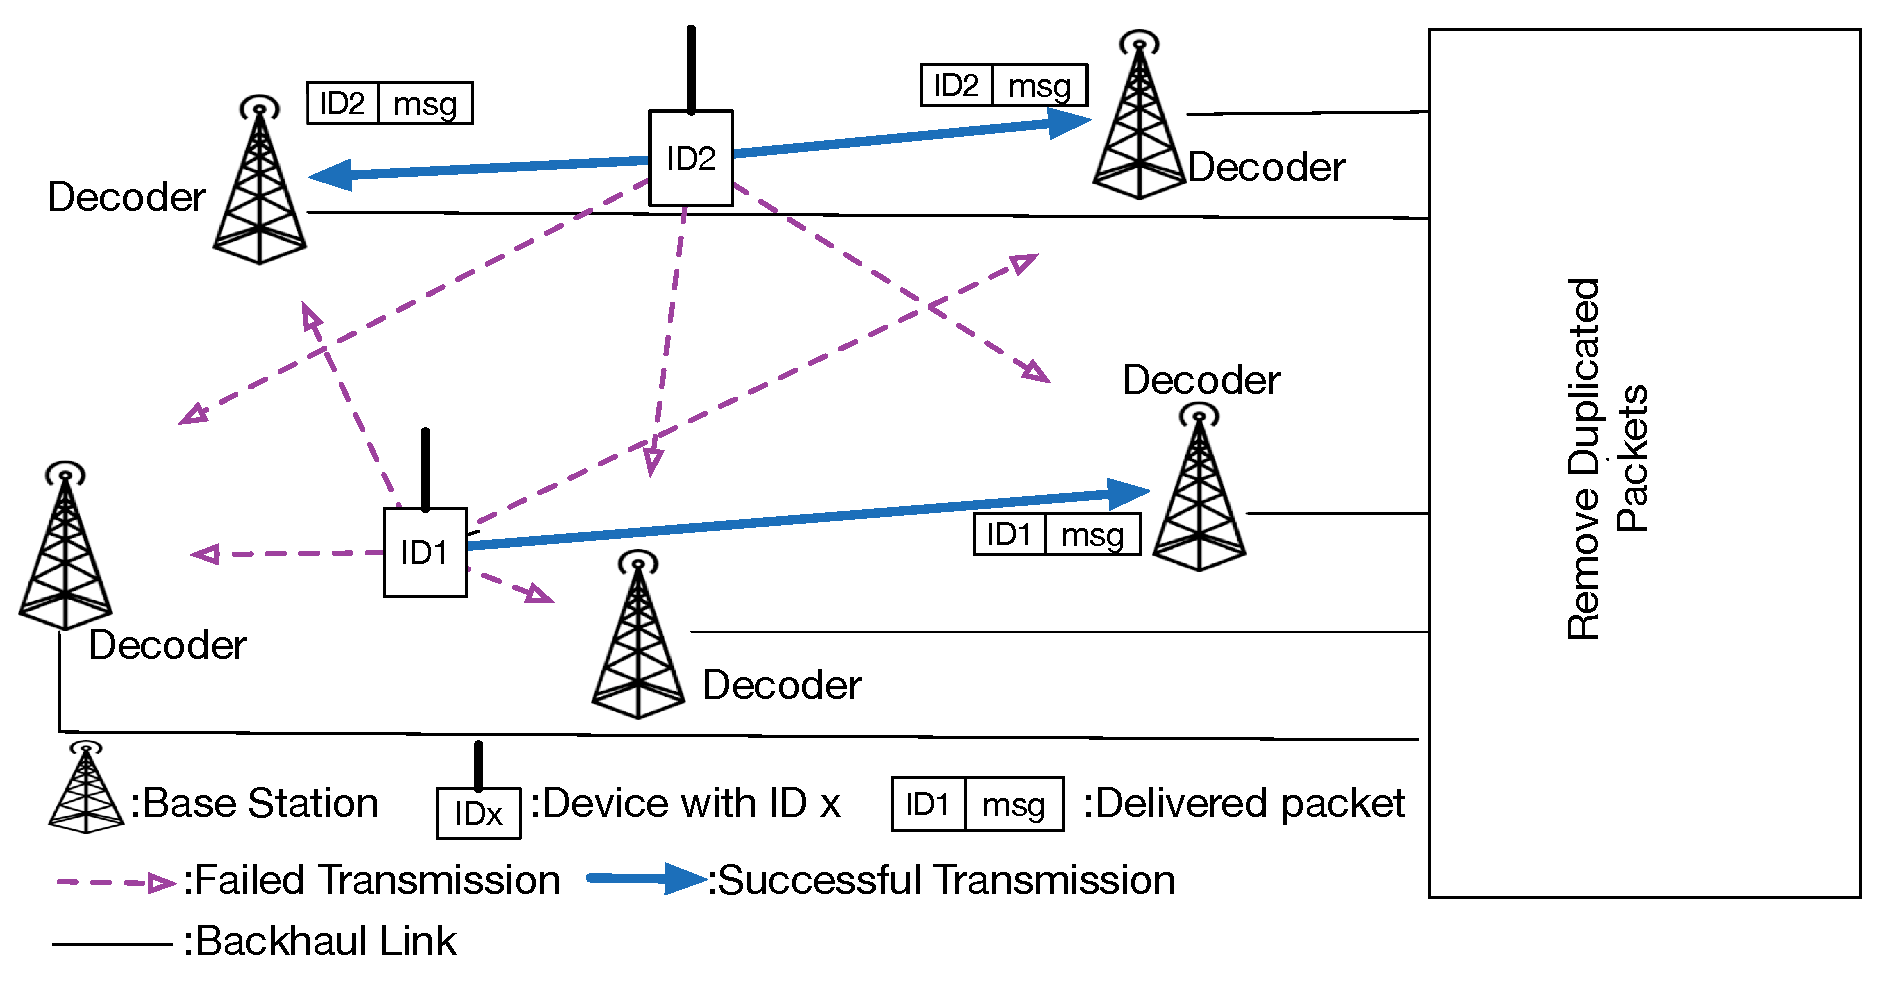
\includegraphics[width=\linewidth]{Chapter5/Figures/Macro_Diversity_Recpetion_Illustration}
	\caption{Macro Reception Diversity Scheme Illustration\qsong{Since we call Maximum Ratio Combining Macro Reception Diversity in anther figure, I'm not sure we should modify the caption of this figure as Selective Combining-like Macro Diversity Reception. Because it is equivalent to judge whether the maximum SINR is greater than captio ratio...}}
	\label{fig:macro_diversity_recpetion_illustration}
\end{figure} 

\begin{figure}[!ht]
	\centering
	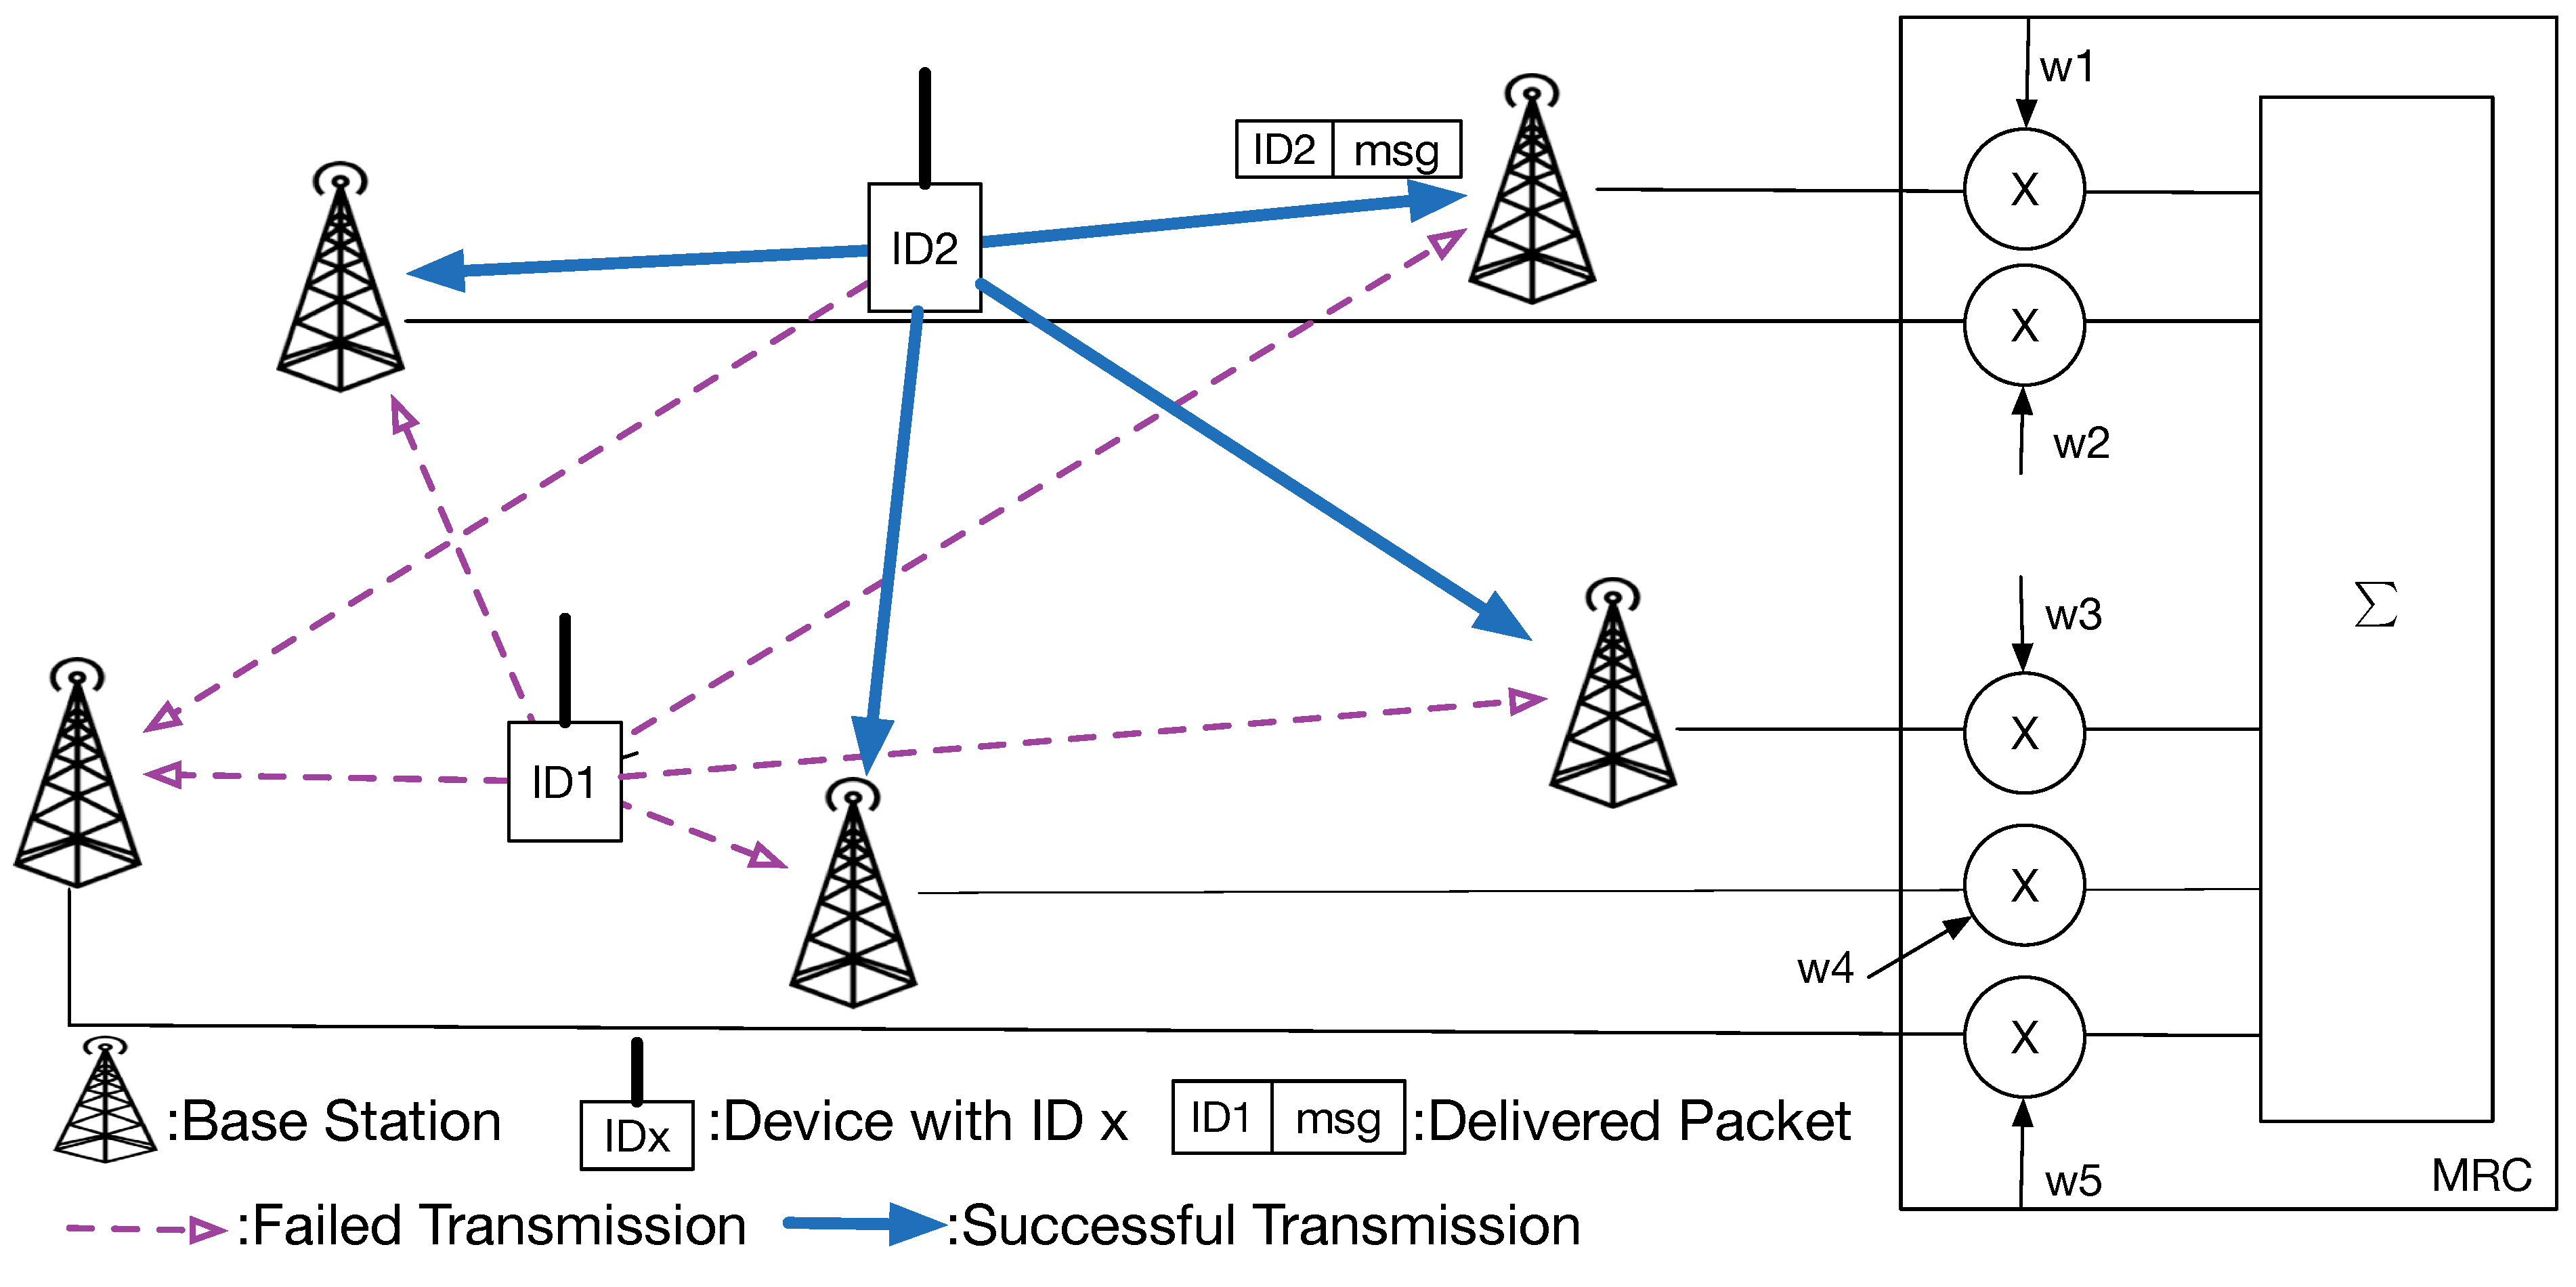
\includegraphics[width=\linewidth]{Chapter5/Figures/MRC_Type_Macro_Diversity_Recpetion_Illustration}
	\caption{Maximum Ratio Combining Macro Reception Diversity Scheme Illustration. The coefficients $w1, w2, ..., w5$ are well designed so that output SINR is maximized.}
	\label{fig:mrc_macro_diversity_recpetion_illustration}
\end{figure} 
%In this broadcast mode, the BSs do not acknowledge the received packets. Hence, the device has to repeat each packet transmission fixed times at random time interval, even if one previous trial is successful. If none of these trials is successful. the packet is lost and the device has no awareness about this. Such a scheme is presently applied by some low-cost dedicated IoT networks, such as SigFox. 

%Not surprisingly, macro reception diversity outperforms the traditional unicast mode in terms of one-shot random access packet loss rate, which means higher system capacity constrained by packet loss rate. However, unicast mode can use retransmission mechanism to reduce packet loss rate while message repeat in macro reception diversity reduces its throughput. 

%In this letter, we propose a simple but accurate analytical model for pure (i.e. non-slotted) and slotted ALOHA based on available stochastic geometry research results. The proposed model takes into account Rayleigh fading, shadowing and capture effect in wireless channel. One can use this model to quantify the macro reception diversity gain in terms of maximum supported load constrained by packet loss rate. 

%derive how many times devices macro reception diversity can serve more that the unicast mode, in a commonly agreed system model. We call the latter performance metric as macro diversity gain.